% Compile with lualatex (see ../writing thesis/latexmkrc for reference settings)
\PassOptionsToPackage{unicode}{hyperref}
\documentclass[aspectratio=1610, 10pt]{beamer}

\usepackage[english]{babel}
\usepackage{csquotes}

\usepackage{amsmath}
\usepackage{amssymb}
\usepackage{mathtools}
\usepackage{siunitx}
\usepackage{booktabs}
\usepackage{graphicx}

\usepackage{hyperref}
\usepackage{bookmark}

% load the theme after all packages
\usetheme[
  showtotalframes,
]{tudo}

\unimathsetup{
  math-style=ISO,
  bold-style=ISO,
  nabla=upright,
  partial=upright,
  mathrm=sym,
}

\DeclareSIUnit\parsec{pc}

\title{Probing Fast Radio Burst Environments}
\subtitle{Cross-Correlating Deep and Shallow FRB Surveys with KiDS DR5}
\author[W.~Ruppert]{Will Ruppert}
\institute[Astroparticle Physics]{Faculty of Physics, TU Dortmund}
\date{2026}
\titlegraphic{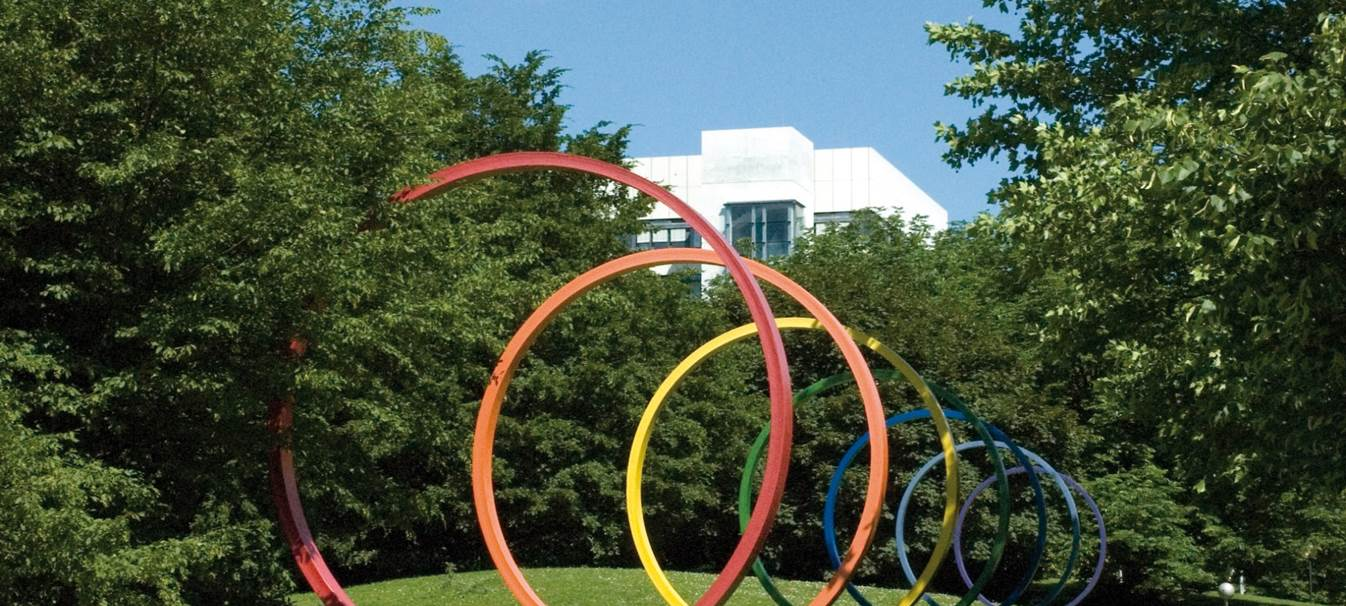
\includegraphics[width=0.55\textwidth]{images/tudo-title-2.jpg}}

\begin{document}

\maketitle

% ---------------------------------------------------------------
\begin{frame}{Motivation}
  \begin{itemize}
    \item Fast Radio Bursts (FRBs) are millisecond-duration radio transients of cosmological origin
    \item Thousands now known (CHIME/FRB: 4539 bursts, 3641 sources), but individual redshifts are rarely measured
    \item Their true progenitors are still unknown -- magnetars vs. delayed neutron-star channels
    \item \textbf{Idea:} cross-correlate the FRB sky distribution with a galaxy survey to statistically infer the FRB redshift distribution and host bias
    \item \textbf{Goal of this thesis:} forecast how well an FRB $\times$ galaxy cross-correlation with KiDS-Legacy can constrain the FRB host-population bias
  \end{itemize}
\end{frame}

% ---------------------------------------------------------------
\begin{frame}{Fast Radio Bursts}
  \begin{columns}[T]
    \begin{column}{0.55\textwidth}
      \begin{itemize}
        \item Bright, ms-duration radio pulses, first discovered in 2007 (Lorimer Burst)
        \item Dispersion measure $DM \propto \int n_e\, \mathrm{d}l$ reveals cosmological (extragalactic) distances
        \item Some sources repeat, others appear as one-off events
        \item Sky distribution consistent with an isotropic, extragalactic population
      \end{itemize}
    \end{column}
    \begin{column}{0.45\textwidth}
      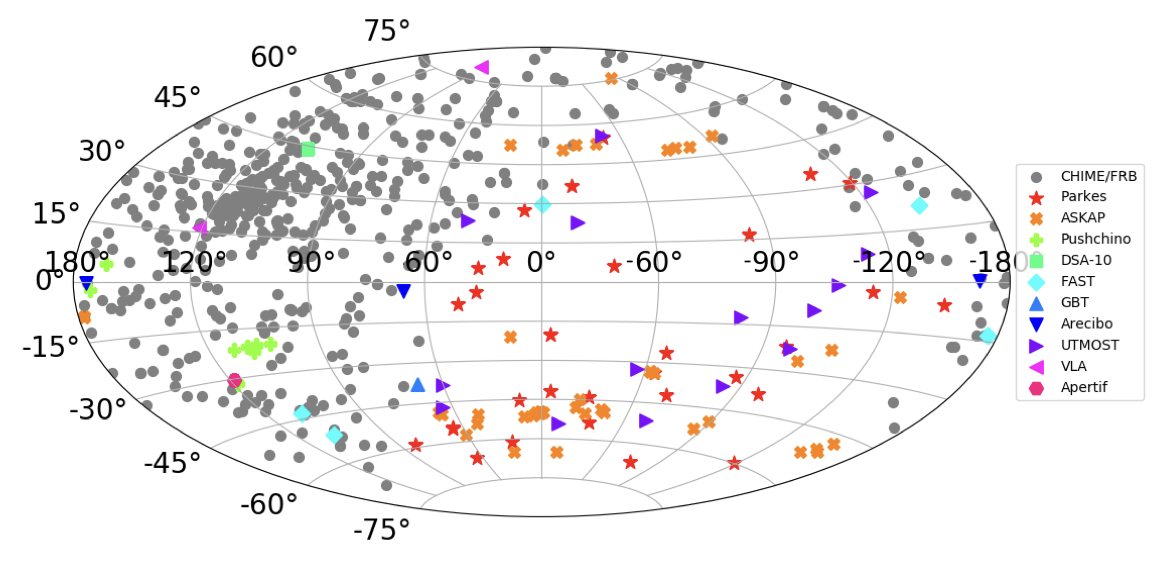
\includegraphics[width=\textwidth]{../programming/frb-cosmology/plots/frb/frb_sky_distribution_petroff.png}
    \end{column}
  \end{columns}
\end{frame}

% ---------------------------------------------------------------
\begin{frame}{Progenitor Models \& Host Bias}
  \begin{columns}[T]
    \begin{column}{0.55\textwidth}
      \begin{itemize}
        \item \textbf{Magnetars}: young neutron stars from core-collapse supernovae, tracking the cosmic star-formation history
        \item \textbf{Delayed neutron stars}: formed via mergers/AIC, with broad delay-time distributions
        \item The two classes predict distinct redshift evolutions, encoded as a linear bias
        \[ b(z) = b_0\,(1+z)^{\delta} \]
        \item Distinguishing them is a key open question in FRB astrophysics
      \end{itemize}
    \end{column}
    \begin{column}{0.45\textwidth}
      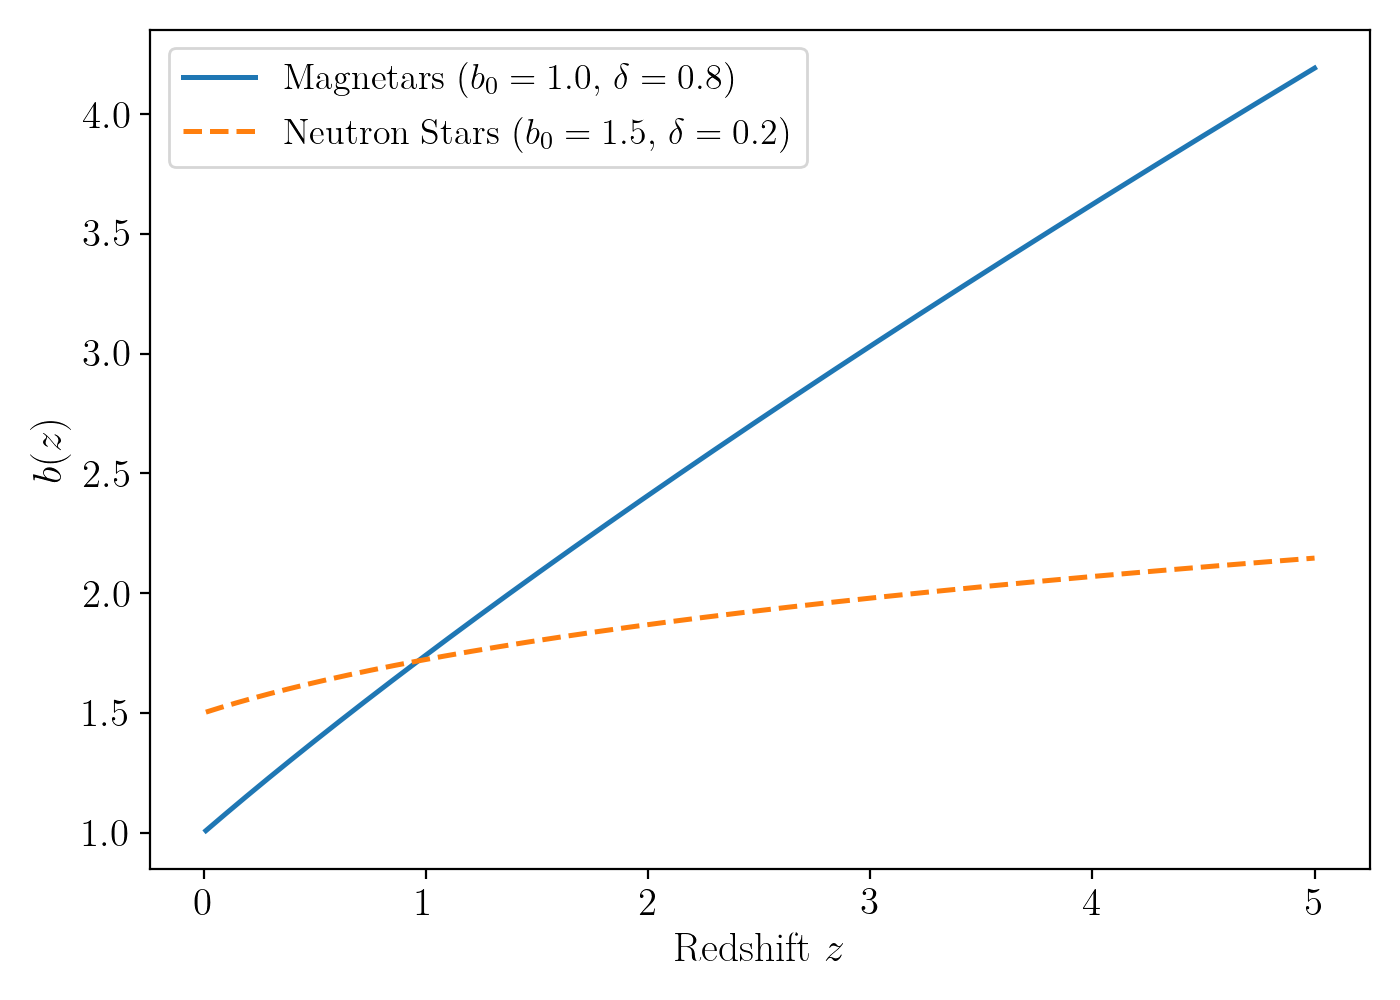
\includegraphics[width=\textwidth]{../programming/frb-cosmology/plots/frb/FRB_bias_bz.png}
    \end{column}
  \end{columns}
\end{frame}

% ---------------------------------------------------------------
\begin{frame}{Angular Power Spectra \& the Limber Approximation}
  \begin{itemize}
    \item Clustering of a tracer field is quantified by the angular power spectrum $C_\ell^{AB}$
    \item Full projection integral reduces, for $\ell \gtrsim \mathcal{O}(10)$, to the Limber approximation
    \[
      C_{\ell}^{AB} \approx \int \frac{\mathrm{d}\chi}{\chi^2}\, W^{A}(\chi)\, W^{B}(\chi)\, P\!\left(k=\frac{\ell+1/2}{\chi},\, z(\chi)\right)
    \]
    \item Radial weight functions $W(\chi) = b(z)\,n(z)\,H(z)/c$ combine the tracer's redshift distribution and bias
    \item Auto-spectra ($A=B$) receive an additive Poisson shot-noise term $N_\ell = 1/\bar{n}$; cross-spectra are shot-noise free
  \end{itemize}
\end{frame}

% ---------------------------------------------------------------
\begin{frame}{Data \& Fiducial Model}
  \begin{columns}[T]
    \begin{column}{0.5\textwidth}
      \textbf{FRB mock samples}
      \begin{itemize}
        \item $n(z) \propto z^2 e^{-\alpha z}$
        \item Shallow: $\alpha=3.5$, $N=5000$
        \item Deep: $\alpha=2.0$, $N=50\,000$
        \item $f_{\mathrm{sky}}=0.9$ for both
      \end{itemize}
      \textbf{Galaxy sample}
      \begin{itemize}
        \item KiDS-Legacy (DR5), $\qty{1347}{\deg\squared}$
        \item 6 tomographic redshift bins
      \end{itemize}
    \end{column}
    \begin{column}{0.5\textwidth}
      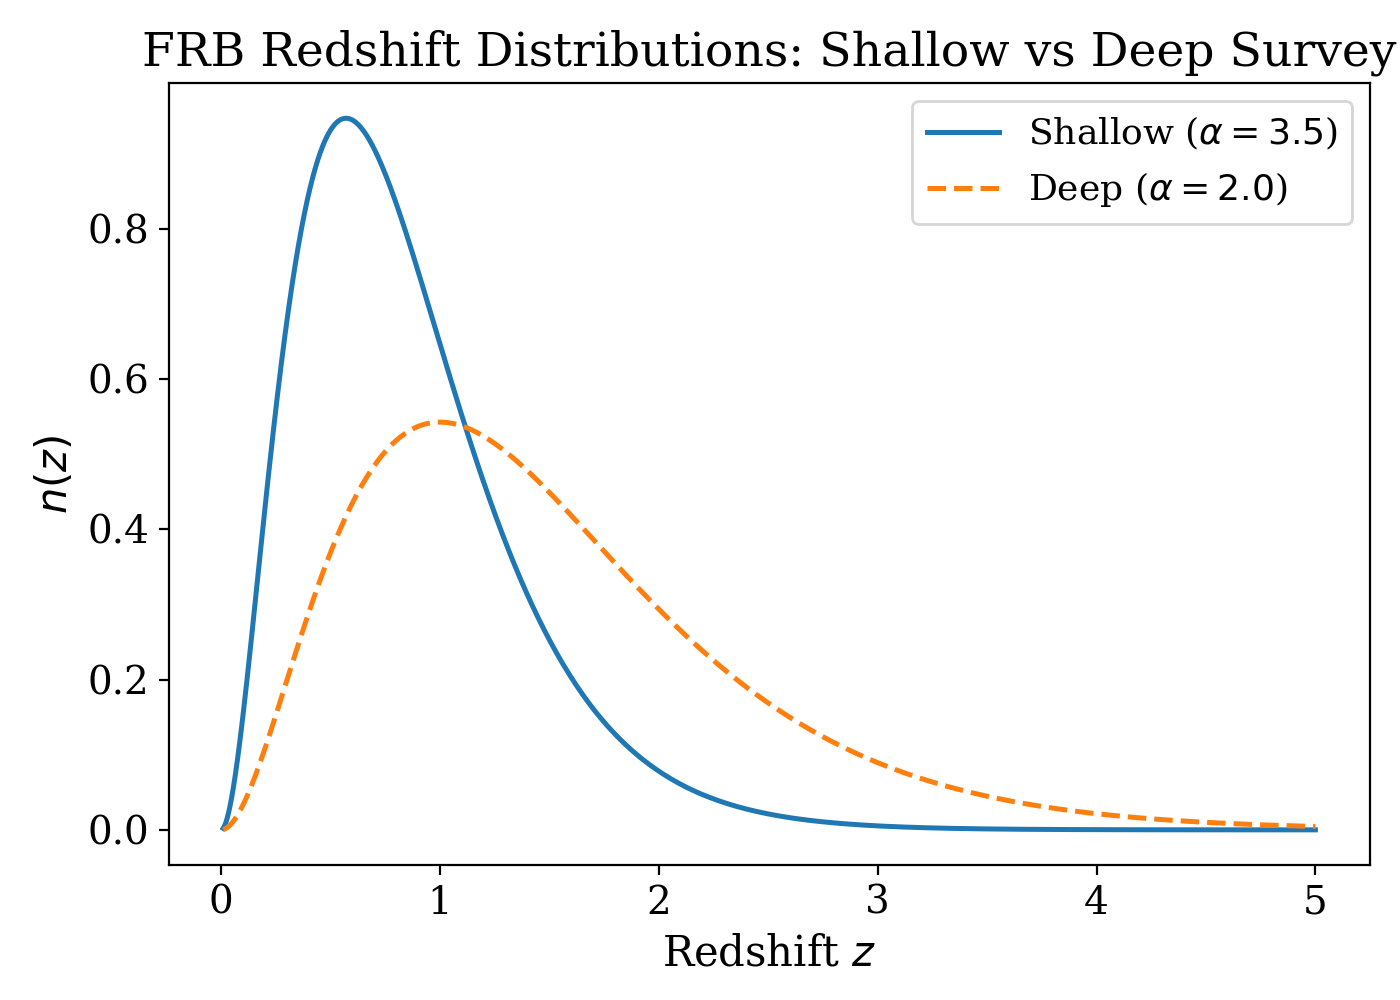
\includegraphics[width=\textwidth]{../programming/frb-cosmology/plots/frb/FRB_nz_shallow_deep.png}\\
      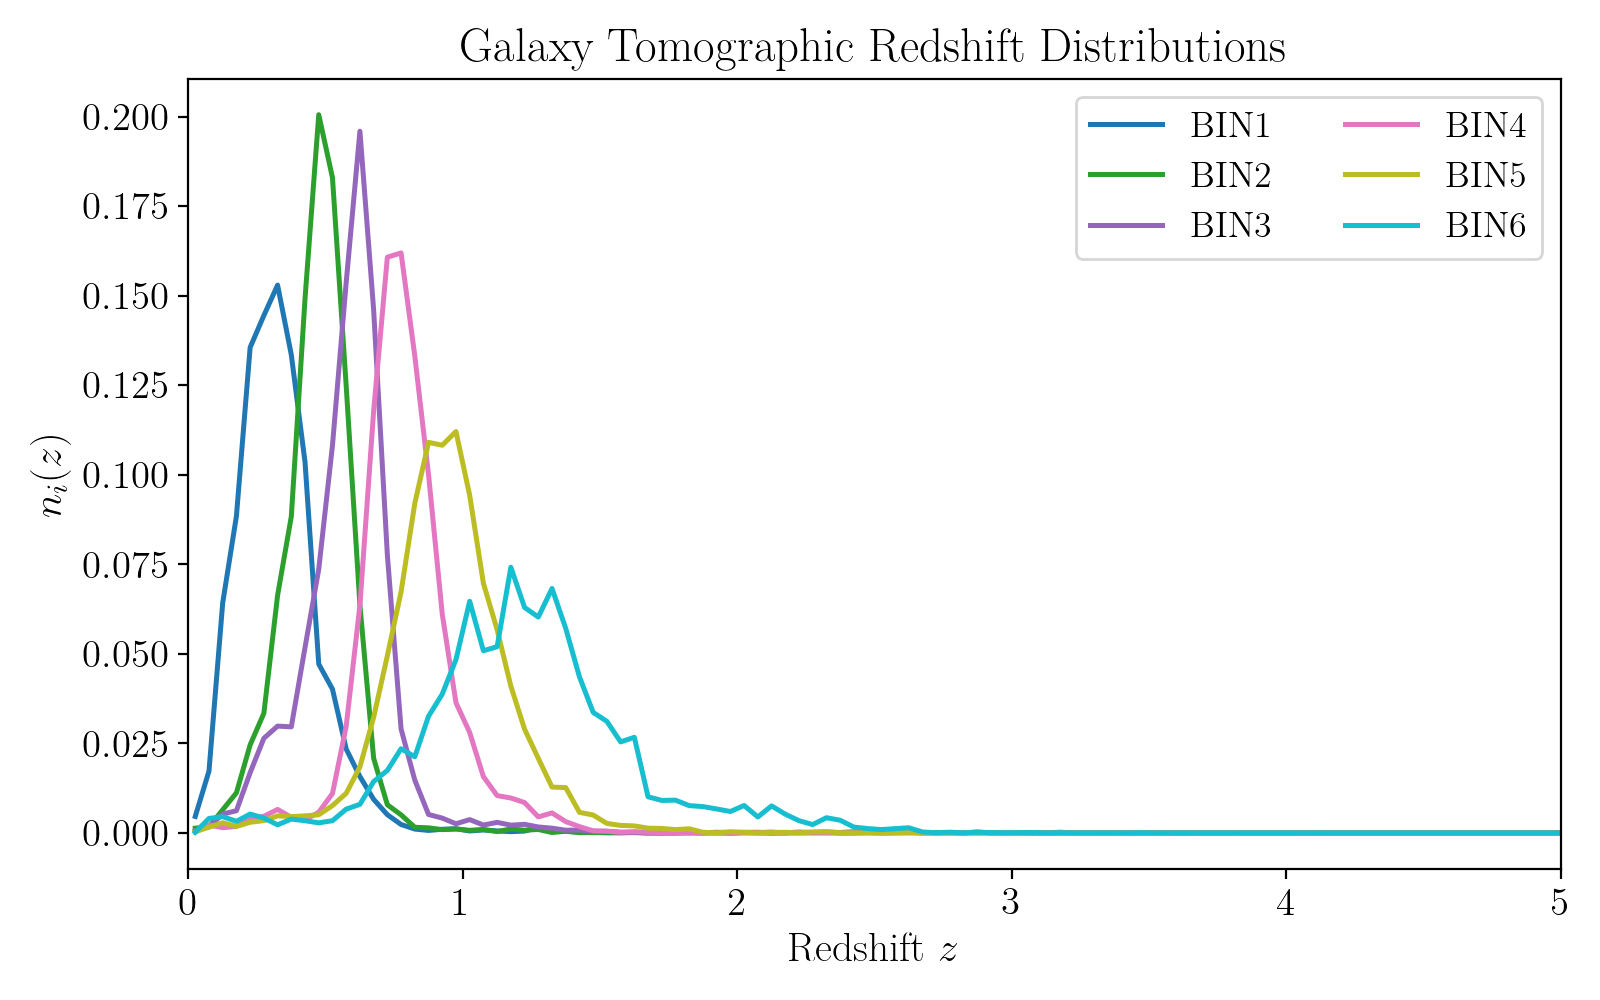
\includegraphics[width=\textwidth]{../programming/frb-cosmology/plots/galaxy/Galaxy_nz_bins.png}
    \end{column}
  \end{columns}
\end{frame}

% ---------------------------------------------------------------
\begin{frame}{FRB Auto-Correlation is Shot-Noise Dominated}
  \begin{columns}[T]
    \begin{column}{0.5\textwidth}
      \begin{itemize}
        \item Planck 2018 flat $\Lambda$CDM cosmology, nonlinear $P(k,z)$ from \texttt{hmf}
        \item For a shallow sample of $N=5000$ bursts, shot noise exceeds the clustering signal by $\sim 3$ orders of magnitude at all multipoles
        \item The FRB auto-spectrum alone carries essentially \emph{no} bias information
        \item[$\Rightarrow$] motivates cross-correlating with a dense galaxy sample
      \end{itemize}
    \end{column}
    \begin{column}{0.5\textwidth}
      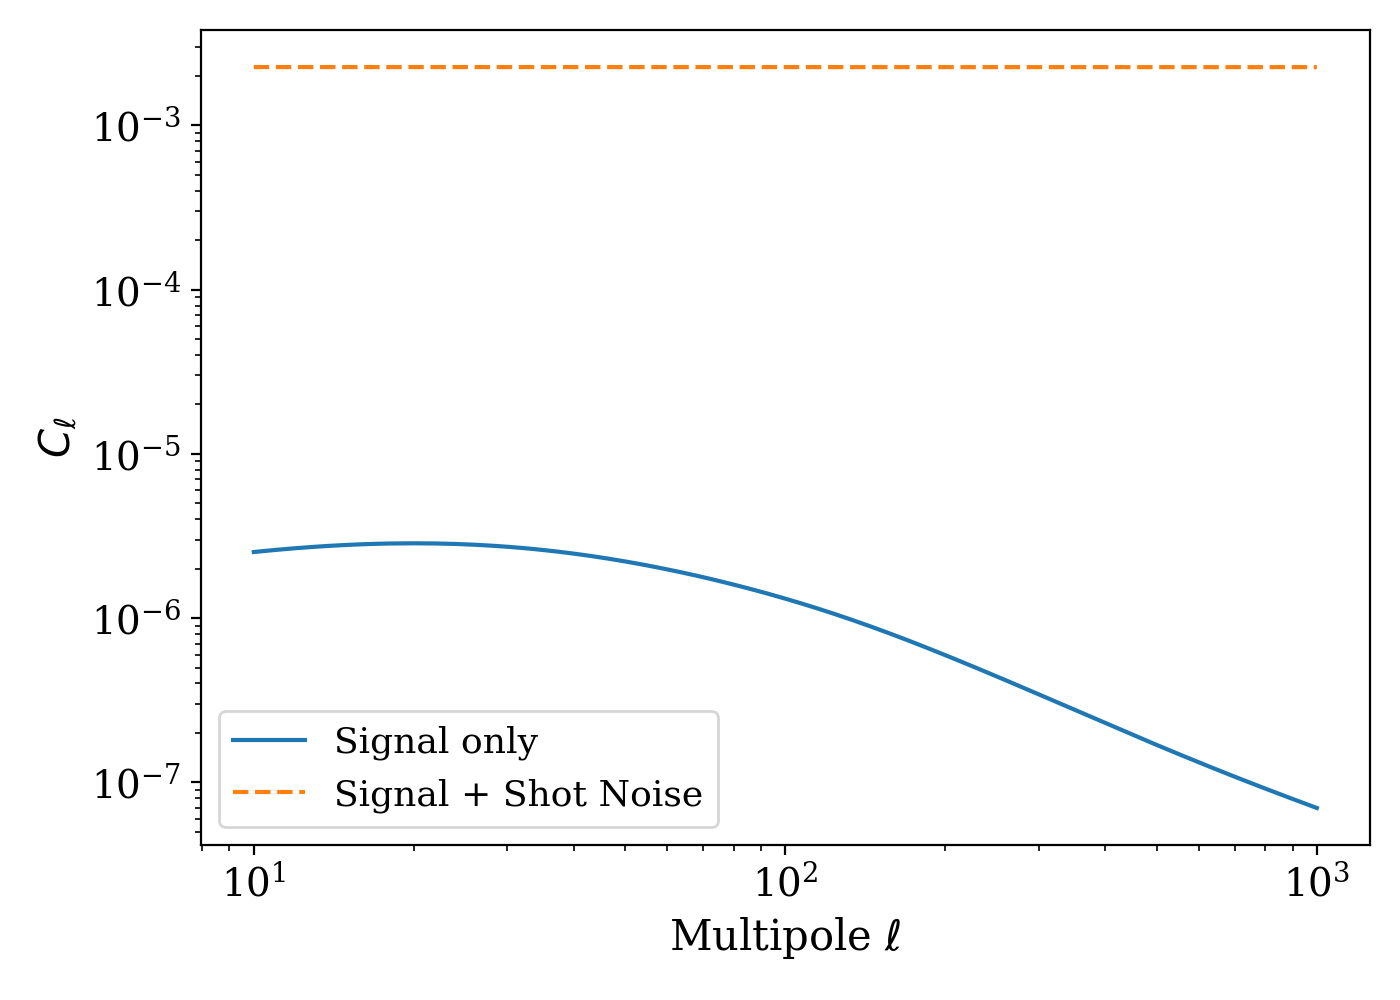
\includegraphics[width=\textwidth]{../programming/frb-cosmology/plots/frb/FRB_magnetar_Cell_shallow_shotnoise.png}
    \end{column}
  \end{columns}
\end{frame}

% ---------------------------------------------------------------
\begin{frame}{FRB $\times$ Galaxy Cross-Spectra}
  \begin{columns}[T]
    \begin{column}{0.5\textwidth}
      \begin{itemize}
        \item Cross-spectra computed for both progenitor classes, both survey depths, and all 6 tomographic bins (24 spectra total)
        \item No shot-noise contamination -- signal set by the radial overlap of FRB and galaxy kernels
        \item Amplitude and shape trace the tomographic bin index and survey depth
      \end{itemize}
    \end{column}
    \begin{column}{0.5\textwidth}
      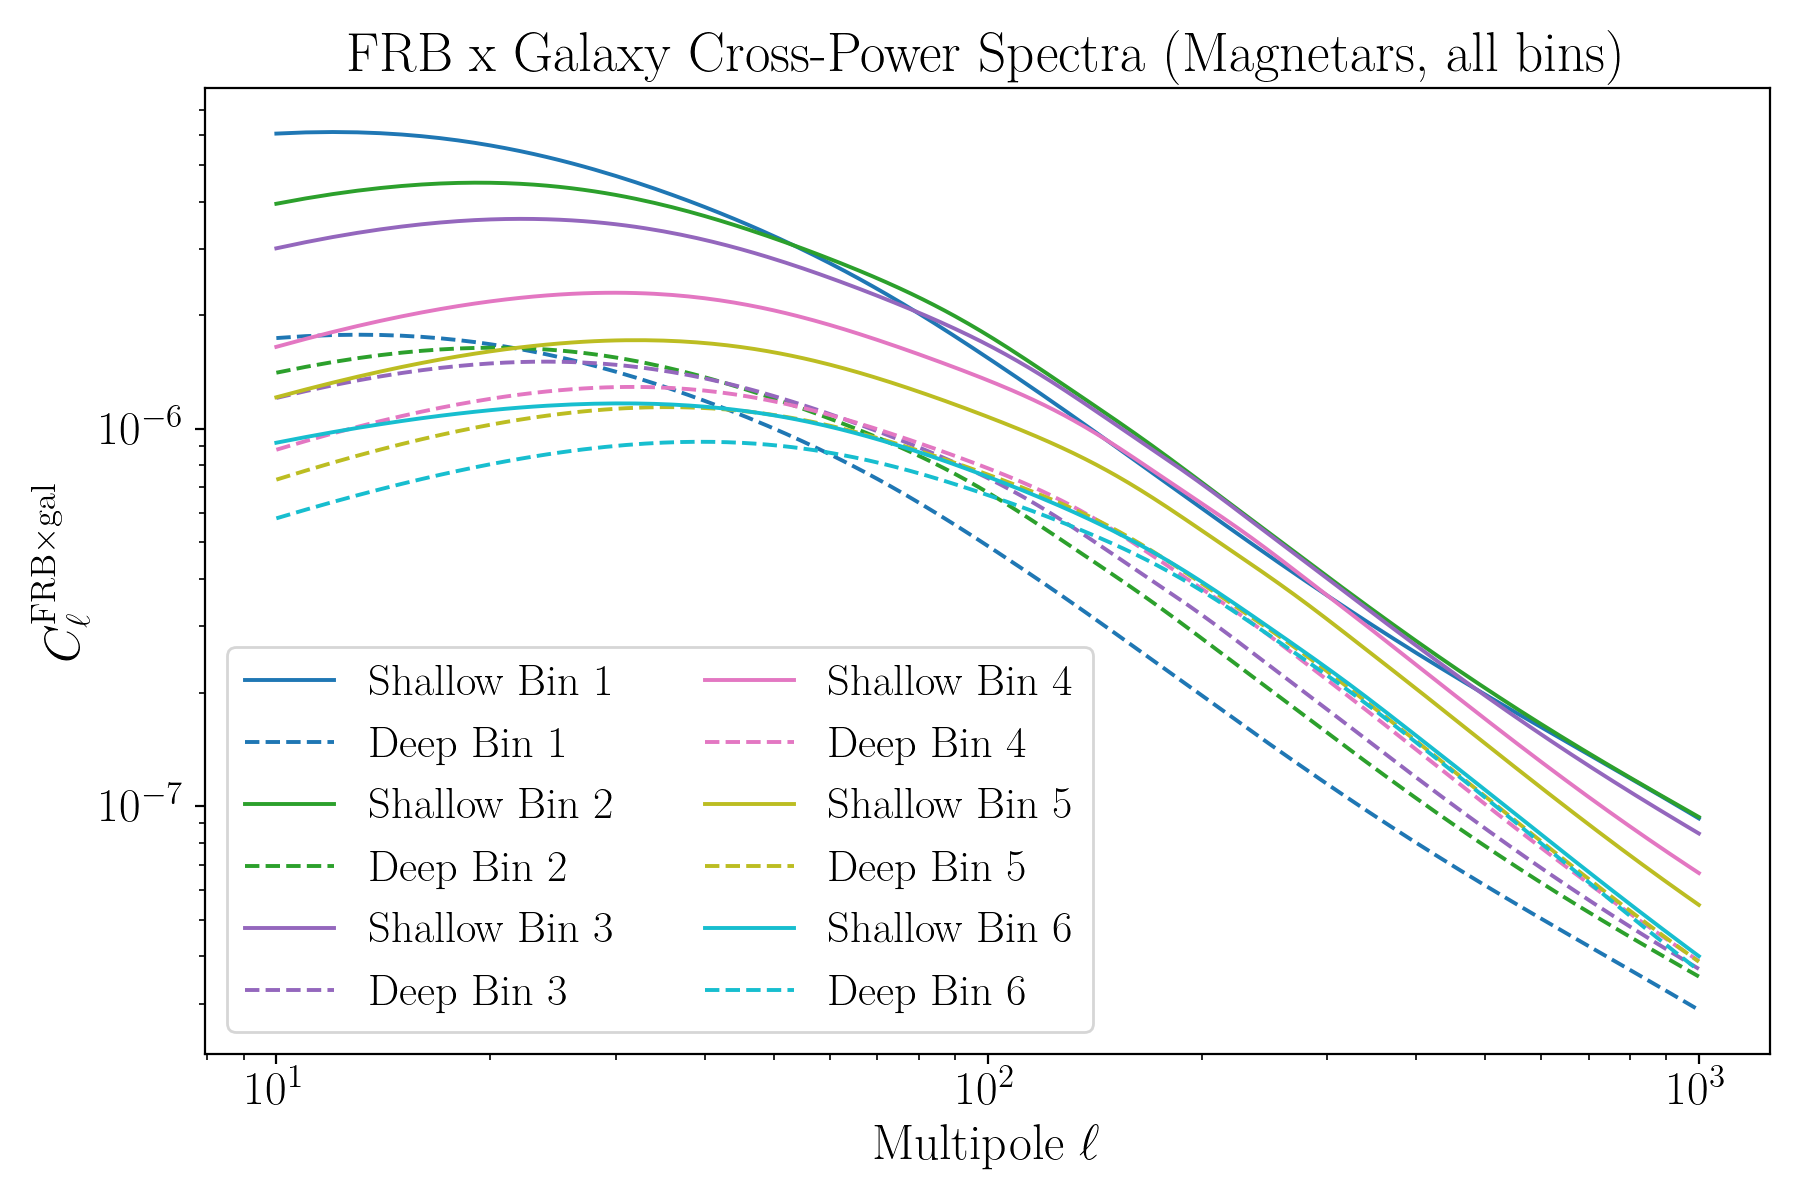
\includegraphics[width=\textwidth]{../programming/frb-cosmology/plots/frb_x_galaxy/comparisons/survey_magnetar_all_bins.png}
    \end{column}
  \end{columns}
\end{frame}

% ---------------------------------------------------------------
\begin{frame}{Fisher Forecast Formalism}
  \begin{itemize}
    \item Gaussian likelihood $\Rightarrow$ parameter covariance from the Fisher matrix
    \[
      F_{ij} = f_{\mathrm{sky}} \sum_{\ell} \frac{2\ell+1}{2}\,
      \operatorname{Tr}\!\left[ C_{\ell}^{-1} \frac{\partial C_{\ell}}{\partial \theta_i} C_{\ell}^{-1} \frac{\partial C_{\ell}}{\partial \theta_j} \right]
    \]
    \item Parameters of interest: FRB bias amplitude $b_0$ and evolution exponent $\delta$
    \item Marginalized errors $\sigma_i = \sqrt{(F^{-1})_{ii}}$; figure of merit $\mathrm{FoM} = 1/\sqrt{\det \mathrm{Cov}}$
    \item Compared: FRB-only ($f_{\mathrm{sky}}=0.9$) vs. joint FRB $\times$ KiDS ($f_{\mathrm{sky}}=0.0327$)
  \end{itemize}
\end{frame}

% ---------------------------------------------------------------
\begin{frame}{Forecast Constraints}
  \begin{columns}[T]
    \begin{column}{0.48\textwidth}
      \small
      \begin{itemize}
        \item FRB-only: $\sigma_{b_0} \approx 23$--$101$ (uninformative)
        \item Joint FRB $\times$ galaxy: $\sigma_{b_0} \approx 1.3$--$2.4$
        \item Improvement: factor $17$--$51$ in $\sigma$, factor $61$--$449$ in FoM
        \item Deep configuration always outperforms shallow, but gains saturate once shot noise no longer dominates
      \end{itemize}
    \end{column}
    \begin{column}{0.52\textwidth}
      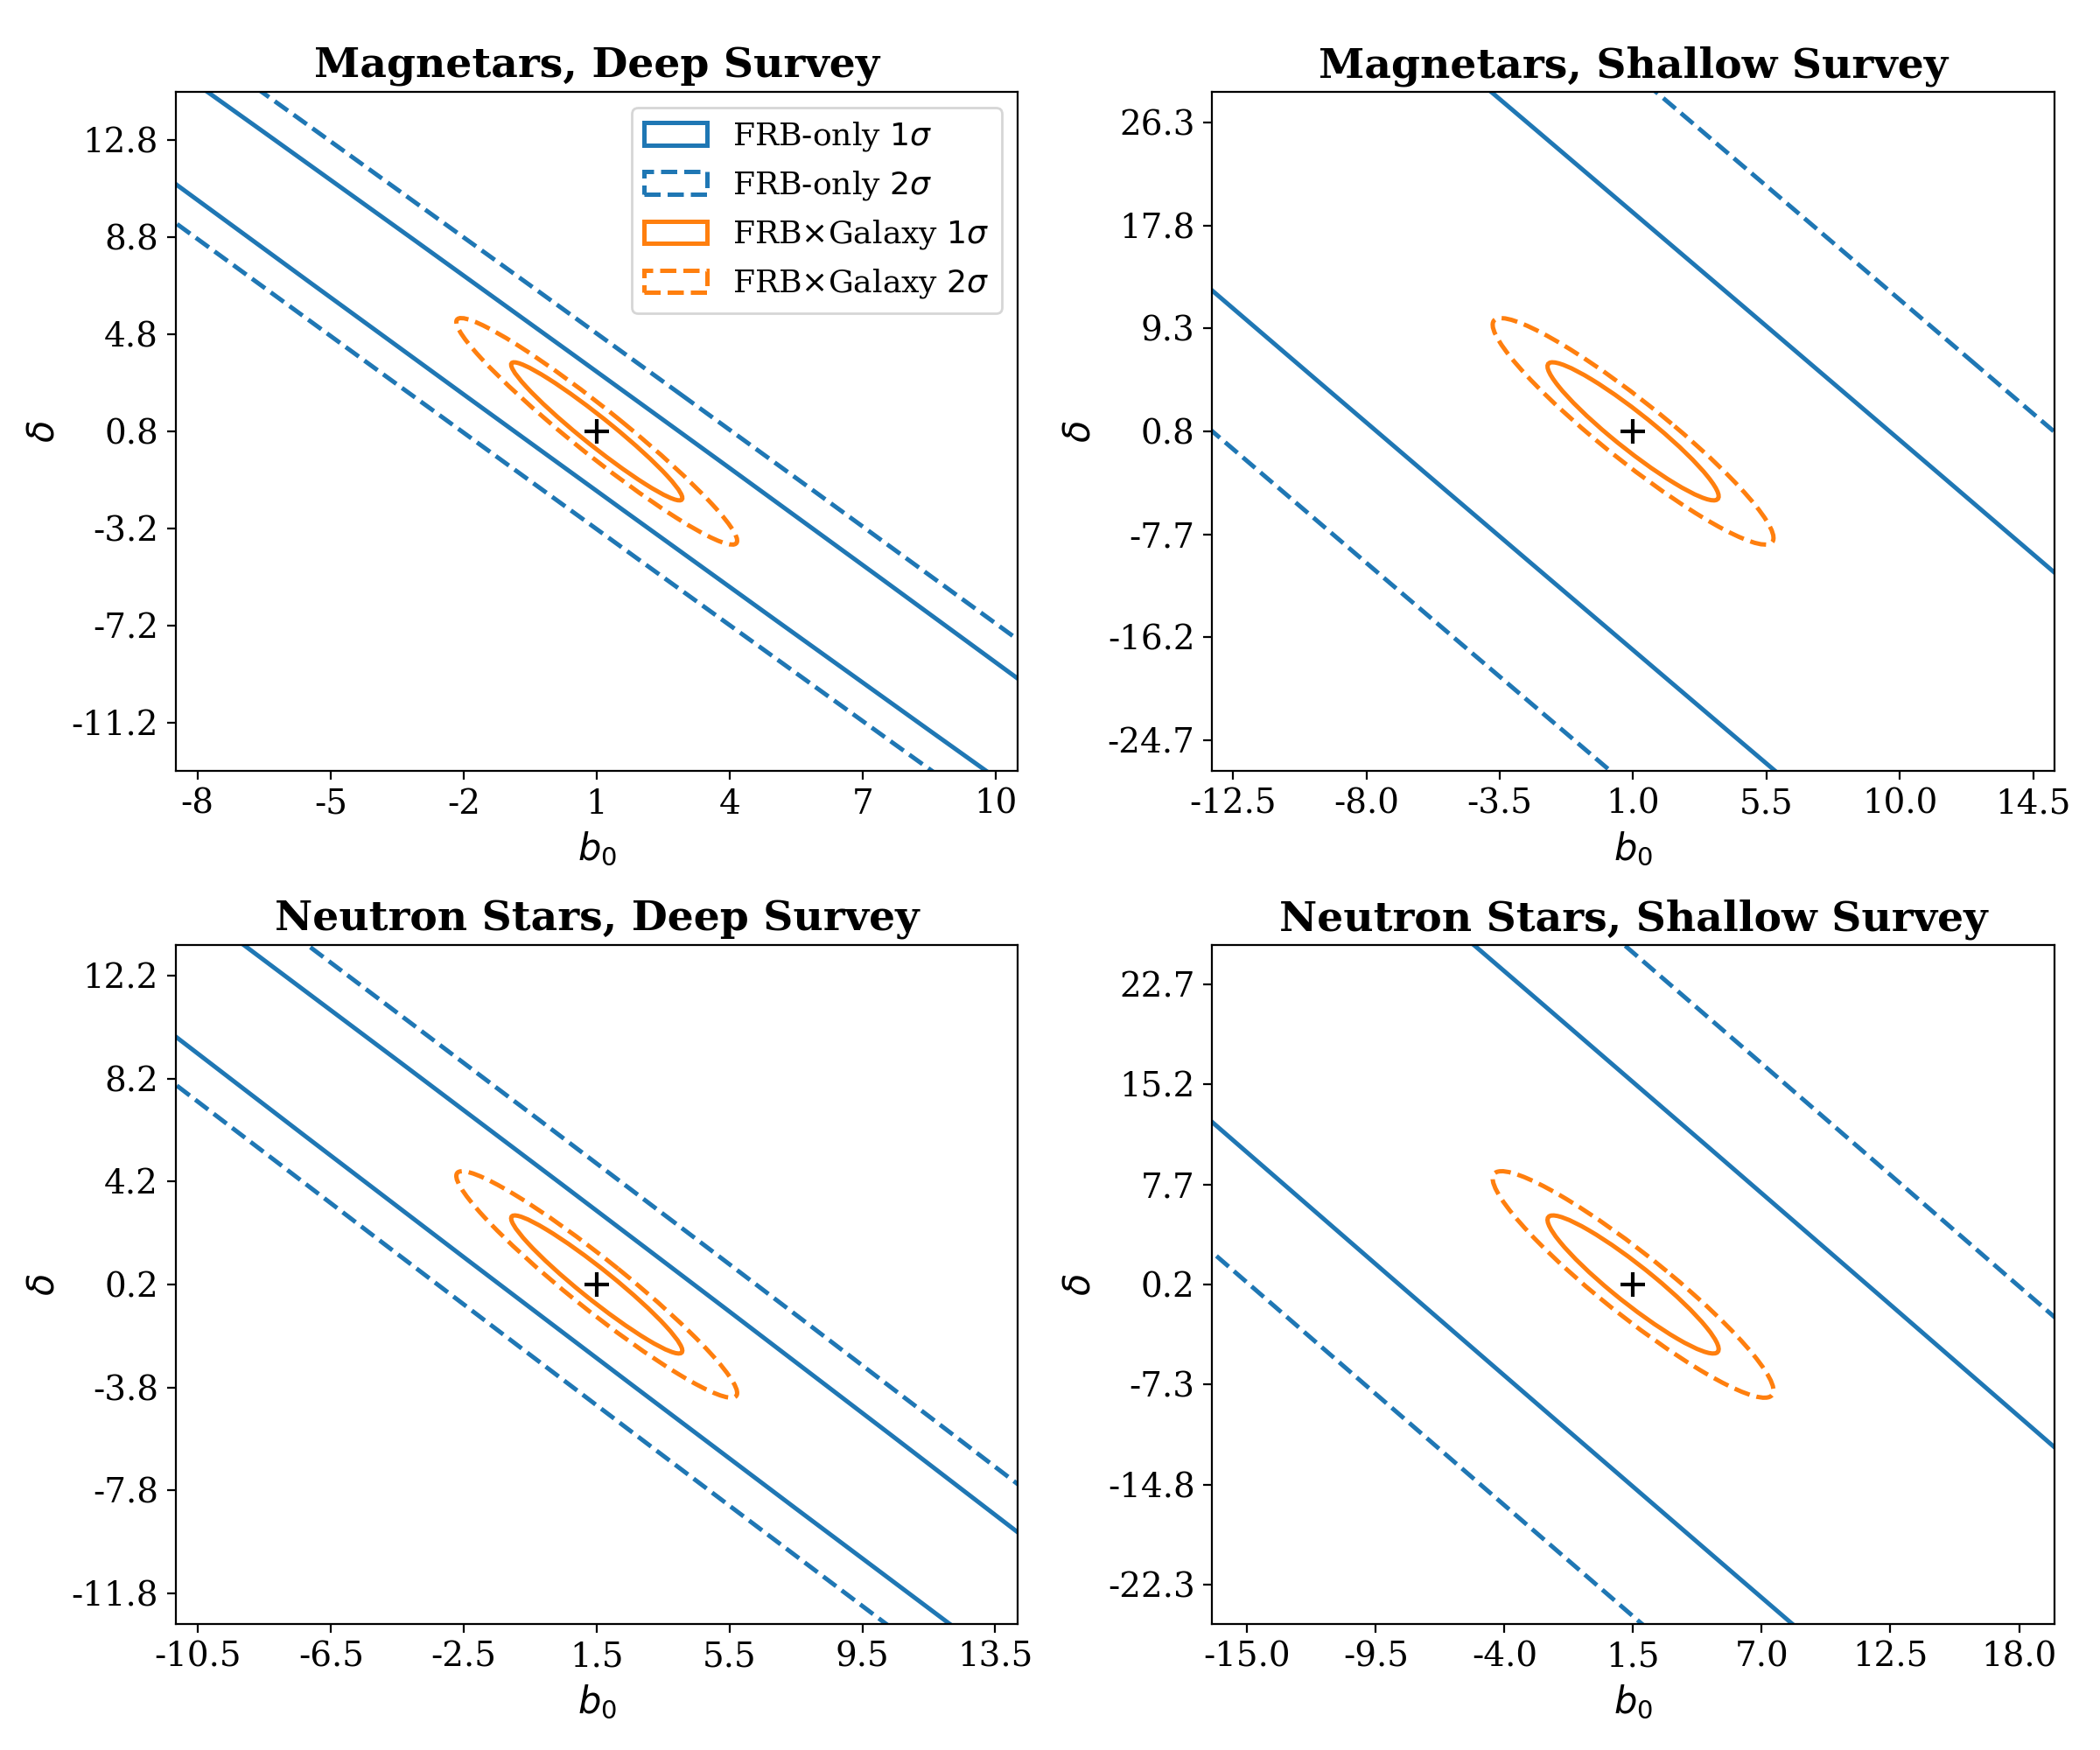
\includegraphics[width=\textwidth]{../programming/frb-cosmology/plots/fisher/fisher_comparison_2x2.png}
    \end{column}
  \end{columns}
\end{frame}

% ---------------------------------------------------------------
\begin{frame}{Discussion}
  \begin{itemize}
    \item Cross-correlation turns an uninformative FRB auto-spectrum into a competitive bias measurement
    \item The two progenitor models ($\Delta b_0 = 0.5$, $\Delta \delta = 0.6$) are \emph{not} yet distinguishable: their fiducial separation lies within the $1\sigma$ joint contour
    \item Fisher information scales linearly with $f_{\mathrm{sky}}$ $\Rightarrow$ sky area is the limiting factor, not burst count
  \end{itemize}
\end{frame}

% ---------------------------------------------------------------
\begin{frame}{Outlook: A Wider Galaxy Survey (LSST)}
  \begin{columns}[T]
    \begin{column}{0.5\textwidth}
      \begin{itemize}
        \item LSST Y10 footprint: $\qty{18000}{\deg\squared}$, $f_{\mathrm{sky}}=0.4363$ ($13\times$ KiDS)
        \item Deep magnetar case: $\sigma_{b_0}$ improves from $1.27 \to 0.25$, FoM $\times 26$
        \item The two progenitor models become distinguishable at $1\sigma$
      \end{itemize}
    \end{column}
    \begin{column}{0.5\textwidth}
      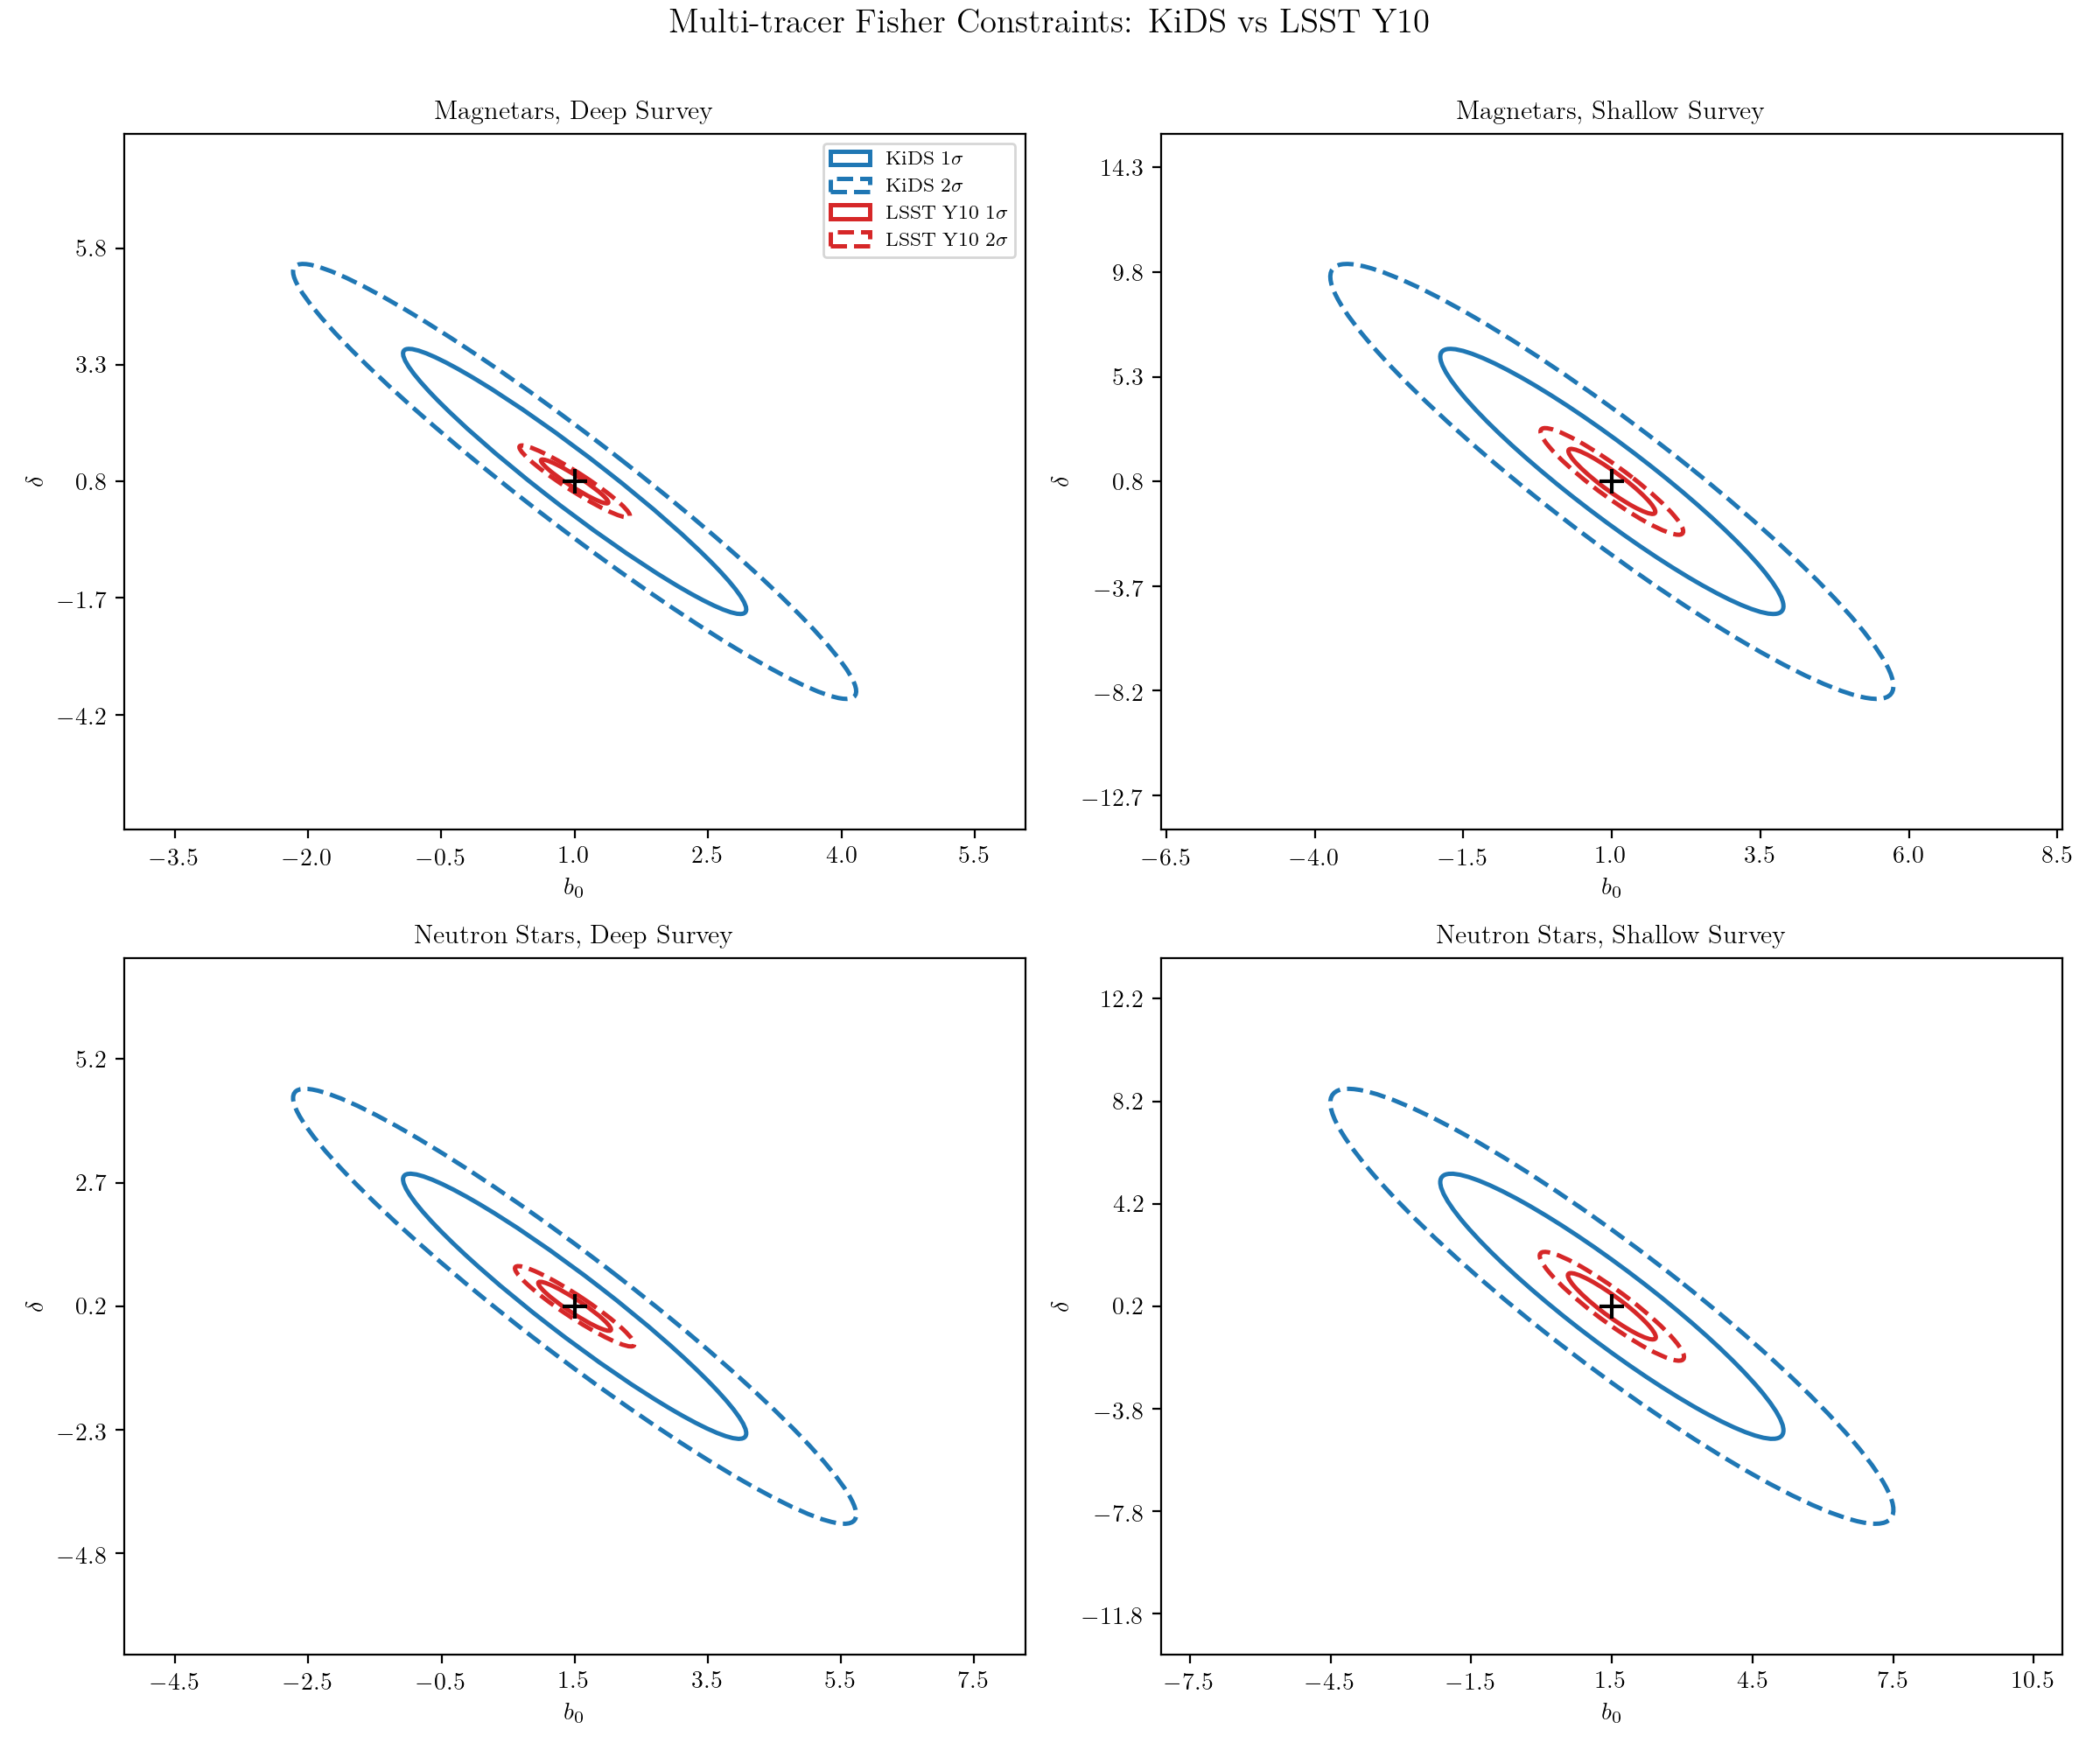
\includegraphics[width=\textwidth]{../programming/frb-cosmology/plots/fisher_lsst/fisher_kids_vs_lsst_2x2.png}
    \end{column}
  \end{columns}
\end{frame}

% ---------------------------------------------------------------
\begin{frame}{Conclusion}
  \begin{itemize}
    \item Built a full forecasting pipeline: matter power spectrum $\to$ radial kernels $\to$ Limber $C_\ell$ $\to$ Fisher forecast
    \item FRB auto-correlation alone is shot-noise dominated and uninformative about host bias
    \item Cross-correlating with KiDS-Legacy improves constraints by $1$--$2$ orders of magnitude
    \item Current footprint is not yet sufficient to separate magnetar vs. neutron-star origin -- but a wider survey such as LSST would be
    \item FRB $\times$ galaxy cross-correlation is a promising probe of FRB host populations
  \end{itemize}
\end{frame}

% ---------------------------------------------------------------
\begin{frame}{Thank You}
  \centering
  \Large Thank you for your attention!\\[1em]
  \normalsize Questions?
\end{frame}

\end{document}
